\newpage
\onecolumn
\appendix
\renewcommand{\thefigure}{A\arabic{figure}}
\renewcommand{\thetable}{A\arabic{table}}
\setcounter{figure}{0}
\setcounter{table}{0}

\section{Appendix}

% ── A.1  Pipeline and Intervention Vocabulary ───────────────────────
\subsection{Pipeline and Intervention Vocabulary}
\label{sec:appendix_pipeline}

\begin{figure}[H]
  \centering
  
\includegraphics[width=0.85\textwidth]{figures/figure_1_pipeline.png}
  \caption{Overview of the lever-based interventional counterfactual
  pipeline.  Each candidate is a structured lever intervention
  $l=(c,s,d,\tau)$.  Phase~1 constructs scene-specific candidates from a
  curated ontology.  Phase~2 performs bounded stochastic generation
  subject to a four-criterion validity audit.  Phase~3 summarises
  accepted edits with auxiliary classifier scoring and, optionally,
  future human pairwise judgements.}
  \label{fig:pipeline}
\end{figure}

\begin{table}[H]
  \centering
  \caption{Intervention vocabulary.  Each concept satisfies all three
  inclusion criteria defined in \S\ref{sec:method}.  Structural
  interventions and social-order cues are excluded as they are not
  realisable under prompt-only editing.}
  \label{sec:intervention_vocabulary}%
  \small
  \begin{tabular}{@{} l l p{5.8cm} @{}}
    \toprule
    Family & Basis & Lever concepts \\
    \midrule
    Physical Maintenance
      & Broken-windows / upkeep~\cite{newman1972,jiang2018brokenwindows}
      & Graffiti removal; litter removal; facade repair; surface cleaning; shutter repair \\[4pt]
    Environmental Amenity
      & Biophilic safety / visibility~\cite{li2015greenery,portnov2020lighting}
      & Localised greenery addition; lighting repair; tree canopy management \\[4pt]
    Visual Legibility
      & Active-frontages / surveillance~\cite{jacobs1961}
      & Signage decluttering; storefront transparency increase \\[4pt]
    Mobility Infrastructure
      & Walkability / road markings~\cite{quintana2025}\textsuperscript{*}
      & Crosswalk repainting; lane marking repainting \\
    \bottomrule
    \multicolumn{3}{@{}l}{\footnotesize\textsuperscript{*}See safety-definition footnote in \S\ref{sec:intro}.}
  \end{tabular}
\end{table}

% ── A.2  Qualitative Examples ───────────────────────────────────────
\subsection{Qualitative Examples}
\label{sec:appendix_qualitative}

\begin{figure}[H]
  \centering
  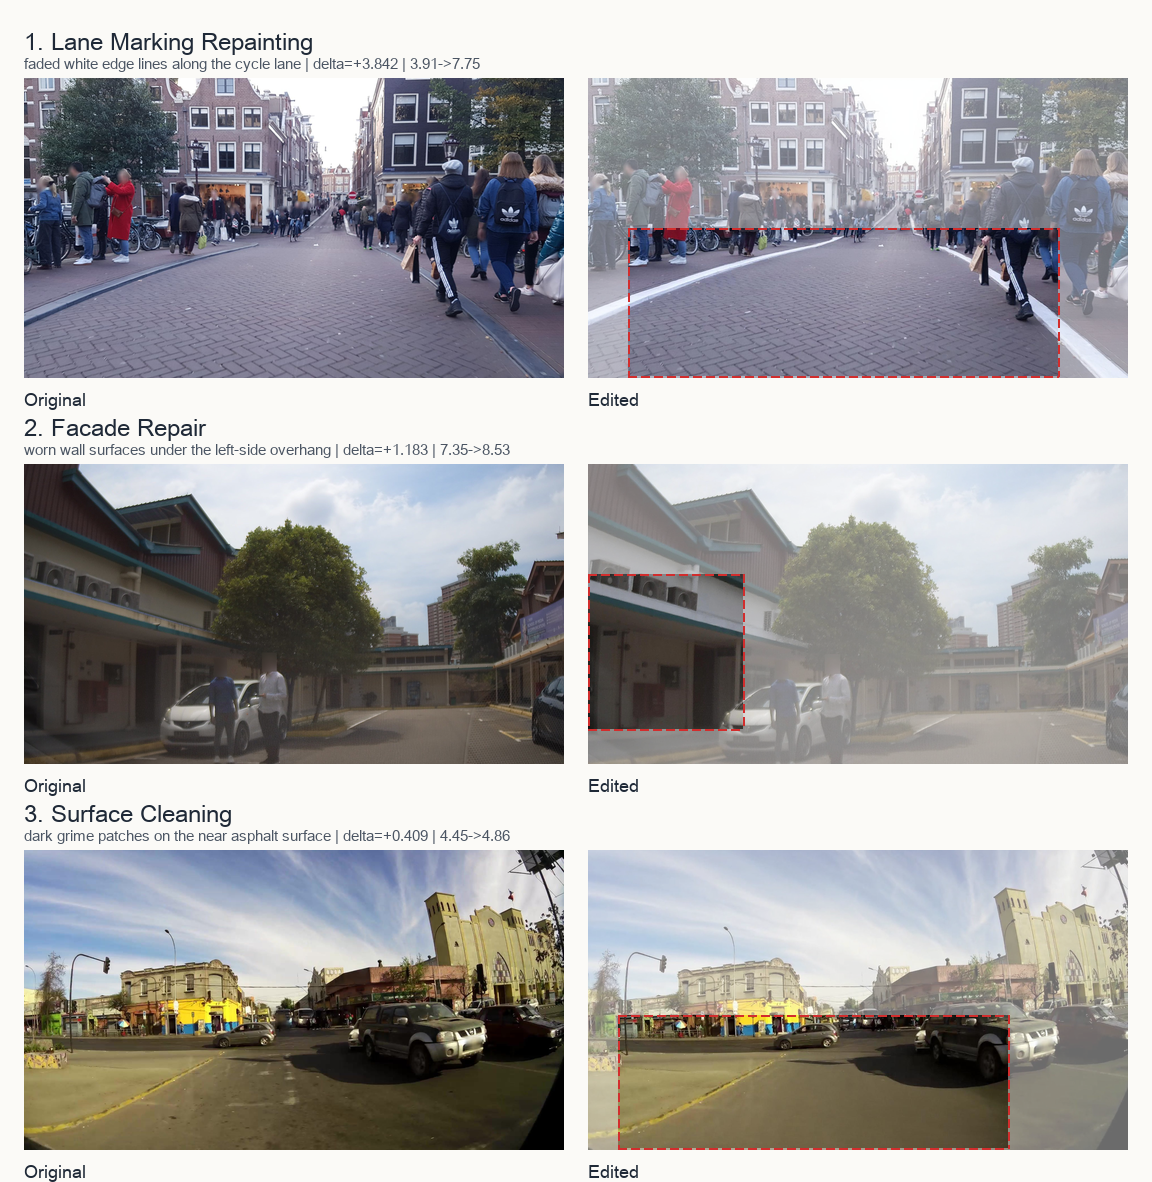
\includegraphics[width=\textwidth]{figures/figure_3_qualitative_highlighted.png}
  \caption{Three qualitative examples from the retained set.
  From top: lane-marking repainting (Amsterdam), facade repair
  (Singapore), surface cleaning (Santiago).  Red dashed bounding boxes
  indicate the edited region; surrounding areas are dimmed for contrast.}
  \label{fig:qualitative}
\end{figure}

% ── A.3  Validity and Coverage Details ──────────────────────────────
\subsection{Validity and Coverage Details}
\label{sec:validity_appendix}

Across 50 scenes the planner produces the full 250 candidate rows
(5.0 per image on average), of which 177 pass the validity audit,
yielding mean coverage $|V(x)|/|L(x)| = 0.708$.
Figure~\ref{fig:distribution} shows the distribution of valid counts per
scene: 2~scenes have one valid lever, 3~have two, 16~have three,
24~have four, and 5~have all five.
The dominant bottleneck is not candidate proposal but valid realisation.
Among the 73 audited-but-rejected edits, plausibility dominates
completely; 45 also show no discernible target change, 25 exhibit
non-local drift, 5 are unrealistic, and none fail same-place
preservation.  Generator failure before audit is zero in the cleaned
$N{=}50$ run, so the remaining variance is concentrated in valid
realisation rather than missing candidate production.

\begin{figure}[H]
  \centering
  \begin{minipage}[t]{0.48\textwidth}
    \centering
    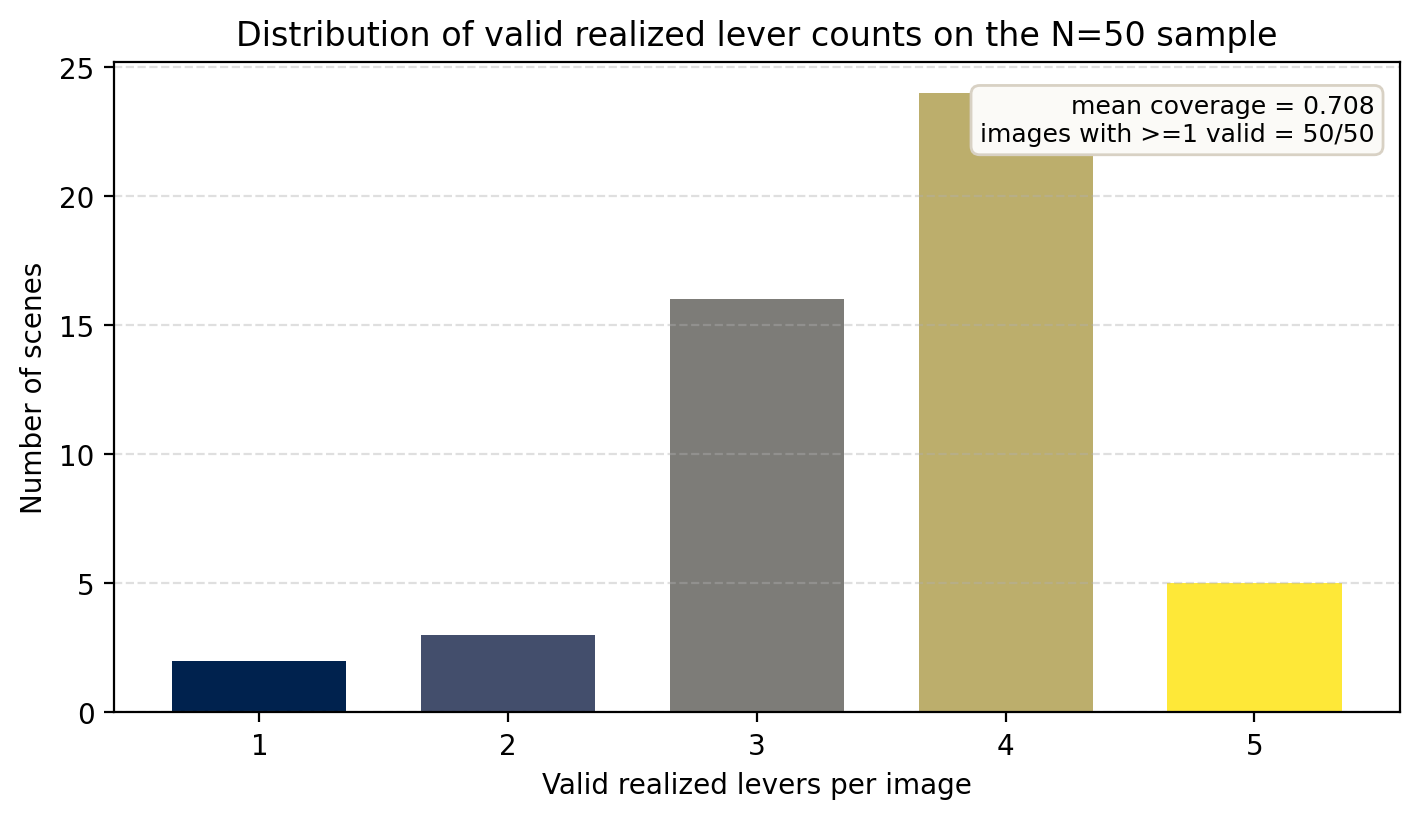
\includegraphics[width=\linewidth]{figures/figure_2_valid_distribution.png}
    \captionof{figure}{Distribution of valid realised lever counts per
    scene ($N{=}50$).  Most scenes admit three or four independently
    valid single-lever interventions.}
    \label{fig:distribution}
  \end{minipage}\hfill
  \begin{minipage}[t]{0.48\textwidth}
    \centering
    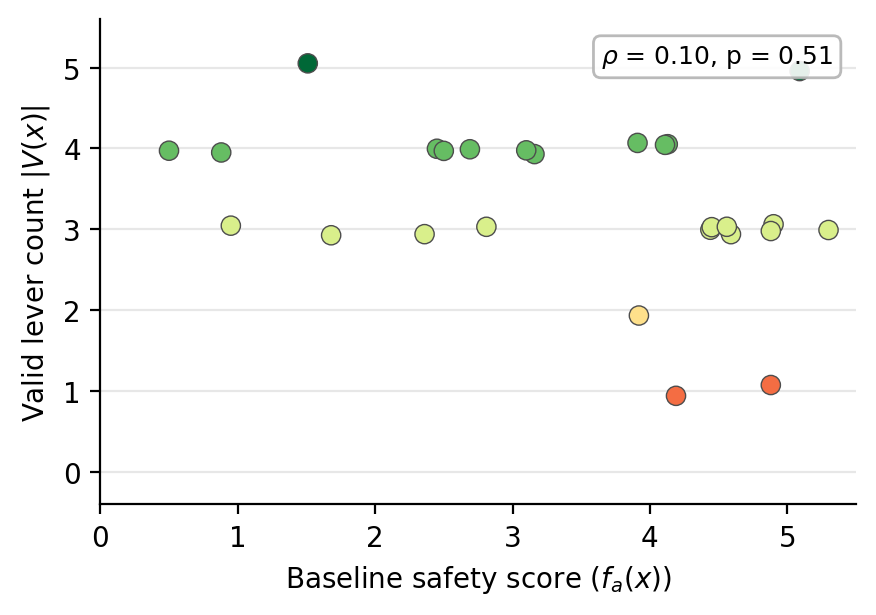
\includegraphics[width=\linewidth]{figures/figure_4_baseline_vs_valid_count.png}
    \captionof{figure}{Baseline safety score vs.\ valid lever count per
    scene ($N{=}50$).  No meaningful relationship is observed
    (Spearman $\rho{=}0.10$, $p{=}0.511$).}
    \label{fig:baseline_vs_valid}
  \end{minipage}
\end{figure}

\begin{table}[H]
  \centering
  \caption{Family-level summary over the full $N{=}50$ run.
  Valid-rate intervals are 95\,\% Wilson confidence intervals; mean
  $\Delta_{\mathrm{aux}}$ and its 95\,\% CI are
  computed over valid edits only.
  $\Delta_{\mathrm{aux}}$ values are on the 0--10 proxy scale.}
  \label{tab:family_appendix}
  \small
  \begin{tabular}{@{} l c c c c @{}}
    \toprule
    Family & Valid / Prop. & Rate [95\,\% CI] & Mean $\Delta_{\mathrm{aux}}$ & $\Delta_{\mathrm{aux}}$ [95\,\% CI] \\
    \midrule
    Physical Maintenance    & 71\,/\,92  & 0.77\,[0.68, 0.85] & $+$0.344 & [$+$0.107, $+$0.584] \\
    Environmental Amenity   & 54\,/\,82  & 0.66\,[0.55, 0.75] & $+$0.287 & [$-$0.041, $+$0.610] \\
    Visual Legibility       &  7\,/\,10  & 0.70\,[0.40, 0.89] & $-$0.177 & [$-$0.927, $+$0.599] \\
    Mobility Infrastructure & 45\,/\,66  & 0.68\,[0.56, 0.78] & $+$0.579 & [$+$0.244, $+$0.923] \\
    \midrule
    \textbf{Overall}        & 177\,/\,250 & 0.71\,[0.65, 0.76] & $+$0.366 & [$+$0.199, $+$0.537] \\
    \bottomrule
  \end{tabular}
\end{table}

\begin{table}[H]
  \centering
  \caption{City-level coverage and directional summary over the full
  $N{=}50$ run.  Each city contributes 10~scenes and therefore
  50~proposed candidates.  Valid-rate intervals are 95\,\% Wilson
  confidence intervals; mean $\Delta_{\mathrm{aux}}$ and its 95\,\% CI
  are computed over valid edits only.
  $\Delta_{\mathrm{aux}}$ values are on the 0--10 proxy scale.}
  \label{tab:city_appendix}
  \small
  \begin{tabular}{@{} l c c c c @{}}
    \toprule
    City & Valid / Prop. & Rate [95\,\% CI] & Mean $\Delta_{\mathrm{aux}}$ & $\Delta_{\mathrm{aux}}$ [95\,\% CI] \\
    \midrule
    Amsterdam     & 40\,/\,50  & 0.80\,[0.67, 0.89] & $+$0.400 & [$+$0.073, $+$0.764] \\
    Abuja         & 32\,/\,50  & 0.64\,[0.50, 0.76] & $-$0.136 & [$-$0.441, $+$0.141] \\
    San Francisco & 36\,/\,50  & 0.72\,[0.58, 0.83] & $+$0.704 & [$+$0.285, $+$1.105] \\
    Santiago      & 38\,/\,50  & 0.76\,[0.63, 0.86] & $+$0.742 & [$+$0.398, $+$1.089] \\
    Singapore     & 31\,/\,50  & 0.62\,[0.48, 0.74] & $-$0.012 & [$-$0.383, $+$0.352] \\
    \midrule
    \textbf{Overall} & 177\,/\,250 & 0.71\,[0.65, 0.76] & $+$0.366 & [$+$0.199, $+$0.537] \\
    \bottomrule
  \end{tabular}
\end{table}

\begin{figure}[H]
  \centering
  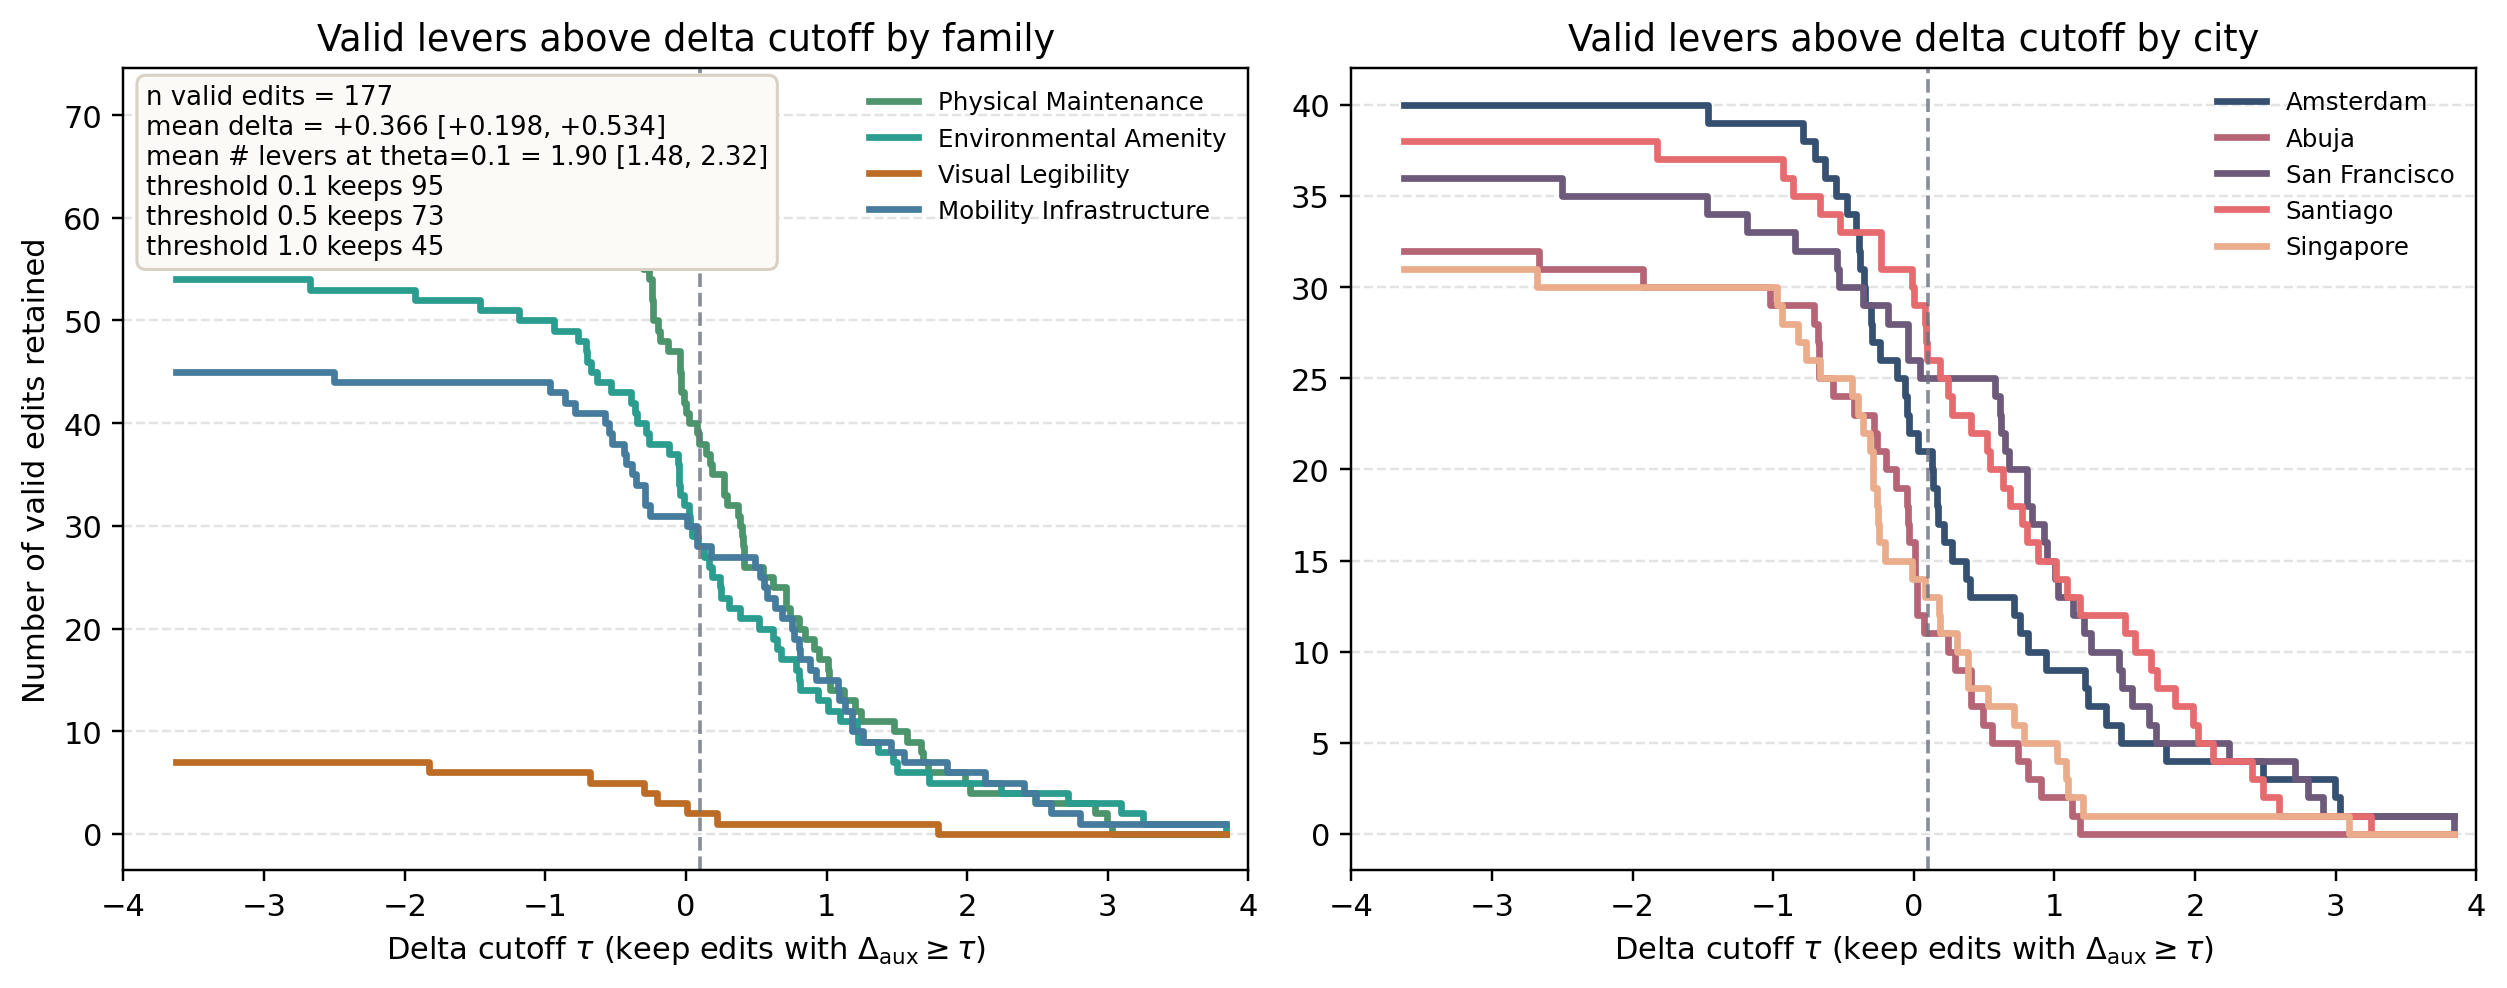
\includegraphics[width=0.85\textwidth]{figures/figure_5_delta_cutoff_counts.png}
  \caption{Average number of retained levers per scene satisfying
  $\Delta_{\mathrm{aux}} \geq \tau$, split by lever family (left) and
  city (right).  The vertical line marks the operating threshold
  $\theta_{\mathrm{aux}}{=}0.1$.  Annotations report the overall mean
  $\Delta_{\mathrm{aux}}$ with 95\,\% CI and the mean number of
  proxy-shortlisted levers per scene with 95\,\% CI.}
  \label{fig:delta_cutoff_counts}
\end{figure}

% ── A.4  Prompt Contracts ───────────────────────────────────────────
\subsection{Prompt Contracts}
\label{sec:prompt_contracts}

The planner, editor, and critic each operate under a structured prompt
contract.  Condensed versions are shown below; full prompts are in the
released repository.

\begin{promptbox}{Planner prompt (condensed)}
\scriptsize\ttfamily
You are an urban perception planner. Given a street-view image and
target percept, propose a constrained set of candidate lever
interventions.\par\medskip
ONTOLOGY: Choose only from four families --- Physical Maintenance,
Environmental Amenity, Visual Legibility, Mobility Infrastructure ---
and prefer cross-family diversity when the scene supports it.\par\medskip
HARD CONSTRAINTS: (1) One lever per candidate. (2) Grounded in a
visible scene element. (3) Local, plausible, prompt-only friendly.
(4) No global relighting, weather, or camera changes. (5) Prefer
the smallest plausible intervention. (6) Exclude theoretically
relevant levers whose target element is not clearly visible/editable
in the image.\par\medskip
DIVERSITY: Return distinct candidates using different lever concepts
and avoid magnitude variants of the same intervention.\par\medskip
Return JSON with field ``candidates'', each containing:
lever\_concept, lever\_family, scene\_support, target\_object,
intervention\_direction, edit\_template, edit\_plan.
\end{promptbox}

\begin{promptbox}{Edit prompt (condensed)}
\scriptsize\ttfamily
Use the PROVIDED image as base. Preserve exact viewpoint, geometry,
and layout.\par\medskip
ALLOWED: Only modify the target object as required by the plan.
If repainting/retexturing, keep shape and placement identical.\par\medskip
FORBIDDEN: No global restyling, relighting, or recoloring. No
adding/removing other objects. No readable text. No background,
sky, road, or context changes.\par\medskip
Lever concept: \{lever\_concept\} \\
Lever family: \{lever\_family\} \\
Scene support: \{scene\_support\} \\
Intervention direction: \{intervention\_direction\} \\
Edit template: \{edit\_template\} \\
Target object: \{target\_object\} \\
Edit plan: \{edit\_plan\}
\end{promptbox}

\begin{promptbox}{Critic prompt (condensed)}
\scriptsize\ttfamily
Evaluate whether the edited image is a valid single-lever
counterfactual relative to the original.\par\medskip
CONTEXT: Edit produced by prompt-only diffusion without masking.
Minor incidental changes (tone drift, texture resampling) are
expected artefacts and should not cause failure unless they
materially alter scene meaning; plausibility and locality are still
judged strictly against the requested lever and support.\par\medskip
CRITERIA:\par\smallskip
(A) edit\_attempted: generator made a visible change at the target
    (false only if output looks identical to original there).\par
(B) same\_place\_preserved: same underlying place.\par
(C) is\_localised: primary meaningful change is in/near intended
    support; minor global tone shifts do not count as non-local.\par
(D) is\_realistic: physically plausible and coherent.\par
(E) is\_plausible: recognisably the requested lever at the stated
    support; fail if the edit type/support is wrong or too
    excessive.\par\medskip
CLEAR FAIL CONDITIONS: Viewpoint/geometry changed; large non-target
objects added/removed; requested lever replaced by a different
change; no discernible change at target.\par\medskip
Return JSON: \{edit\_attempted, same\_place\_preserved,
is\_localised, is\_realistic, is\_plausible, notes\}, where
notes = \{failure\_modes, diagnosis, repair\_suggestion\}.
\end{promptbox}
